\documentclass[a4paper,12pt,final]{article}

\usepackage[italian]{babel}
\usepackage[utf8]{inputenc}   
\usepackage[T1]{fontenc}

\usepackage{graphicx}
\usepackage{subcaption}
\usepackage{hyperref}

\graphicspath{{img/}}

\begin{document}
	\begin{figure}
		\centering
		\begin{subfigure}{0.45\textwidth}
			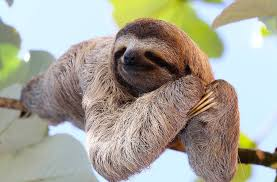
\includegraphics[width=\textwidth]{sloth}
			\caption{A sloth chilling on its branch}
		\end{subfigure}
		\hfill
		\begin{subfigure}{0.45\textwidth}
			
\includegraphics[width=\textwidth]{baby}
			\caption{A smiling (creepy) sloth}
		\end{subfigure}
		
		\begin{subfigure}{0.45\textwidth}
			
\includegraphics[width=\textwidth]{SIdSloth}
			\caption{A prehistoric sloth}\label{fig:sid}
		\end{subfigure}
		\hfill
		\begin{subfigure}{0.45\textwidth}
			
\includegraphics[width=\textwidth]{flash}
			\caption{The fastest sloth ever}
		\end{subfigure}
		\caption{Some images of my spiritual animal: the sloth}\label{fig:sloth}
	\end{figure}
	In \autoref{fig:sloth} troviamo diverse immagini di bradipi. In particolare, quello in \autoref{fig:sid} è Sid.
	
\end{document}